\documentclass[a4paper]{article}
\usepackage[margin=1in]{geometry}
\usepackage[dvipsnames, svgnames, x11names]{xcolor}
\usepackage{ctex, cite, amsfonts, amsmath, graphicx, lipsum, amssymb, url, listings, bm, float, siunitx, framed, color, tikz, booktabs, fontspec, unicode-math, mdframed, tcolorbox, fancyhdr, titling}
\usepackage{minted}
\tcbuselibrary{minted}
\tcbuselibrary{skins, listingsutf8, breakable}
\usepackage[sort&compress]{gbt7714}
\usepackage[colorlinks=true, citecolor=black]{hyperref}
\usepackage{cleveref}
\setmainfont{Times New Roman}
\setsansfont{Arial}
\setmonofont{SpaceMono Nerd Font}
\setCJKmainfont[AutoFakeBold=true]{SimSun}
\setCJKsansfont[AutoFakeBold=3]{楷体}
\setCJKmonofont[AutoFakeBold=3]{SimHei}
\DeclareFontFamily{U}{bbold}{\skewchar\font127 }
\DeclareFontShape{U}{bbold}{m}{n}{
   <-6> bbold5
   <6-8> bbold7
   <8-> bbold10
}{}
\hypersetup{pdftitle={}, pdfauthor={Crazy\_13754}}
% \begin{tcblisting}{listing engine=minted,boxrule=0.1mm,colback=blue!5!white,breakable,colframe=blue!75!black,listing only,left=5mm,minted options={fontsize=\small,breaklines, autogobble,linenos,numbersep=3mm,escapeinside=||},minted language=text}
% \end{tcblisting}
\definecolor{LightGray}{gray}{0.9}
\definecolor{darkgray}{gray}{0.3}

\newmdenv[leftline=true, linecolor=gray, linewidth=2pt, topline=false, bottomline=false, rightline=false, leftmargin=10pt,  font=\sffamily\color{darkgray}]{quoted}

\newtcolorbox{citebox}{boxrule=0pt, left=10mm, right=10mm, top=5mm, bottom=5mm, fonttitle=\bfseries, sharp corners, before skip=10pt, after skip=10pt}
\newcommand{\upcite}[1]{	extsuperscript{\cite{#1}}}
\citestyle{numbers}

\begin{document}

\title{数字电路实验报告——说明文档}
\author{张荣宸、罗浙元、毕冠华}
\date{}

\maketitle
\tableofcontents

\section{核心算法——埃拉托斯特尼筛法}
\subsection{算法原理}

埃拉托斯特尼筛法是一种用来求解素数的算法,其基本思想是从小到大枚举每一个数,如果这个数是素数,那么就将它的所有倍数标记为合数。这样,当枚举到一个数时,如果它没有被标记为合数,那么它就是素数。

其伪代码如下:

\begin{tcblisting}{listing engine=minted,boxrule=0.1mm,colback=blue!5!white,breakable,colframe=blue!75!black,listing only,left=5mm,minted options={fontsize=\small,breaklines, autogobble,linenos,numbersep=3mm,escapeinside=||},minted language=python}
for i = 2 to n:
   if not is_prime[i]:
      continue
   for j = i * i to n step i:
      is_prime[j] = false
\end{tcblisting}

\subsection{算法实现}

在我们的代码中,\texttt{eshelby\_screen} 模块实现了基于状态机的埃氏筛的算法,其状态转移图如 \ref{fig:state.png} 所示。状态机包括以下状态:
\begin{itemize}
   \item \texttt{KILLER\_STATE}:筛选合数状态,将当前素数的倍数标记为合数。
   \item \texttt{CHECK\_PRIME\_STATE}:检查素数状态,检查下一个数是否为素数。
   \item \texttt{READ\_TO\_CHECK\_STATE}:等待 SRAM 读取状态,等待 SRAM 读取下一个数。
   \item \texttt{INITIAL\_STATE}:初始化状态,初始化计数器和 SRAM。
   \item \texttt{DONE\_STATE}:筛选完成状态,筛选完成。
\end{itemize}

\begin{figure}[H]
\centering
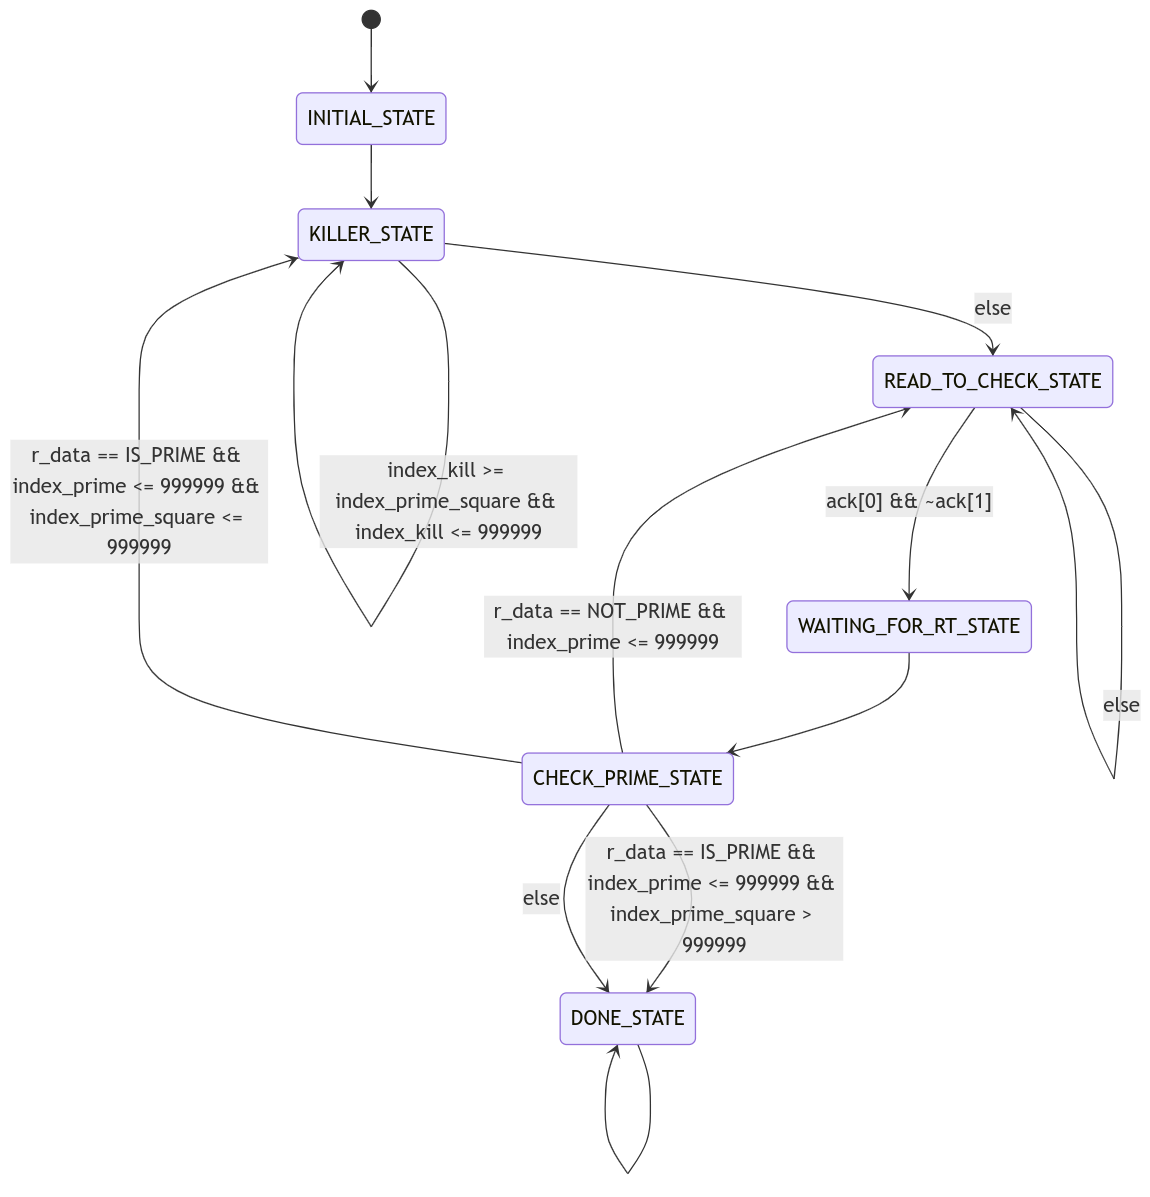
\includegraphics[width=0.8\textwidth]{./image/2/state.png}
\caption{埃拉托斯特尼筛法状态转移图}
\label{fig:state.png}
\end{figure}

我们没有实现多周期除法器,因为在这个算法中我们不需要除法器。我们使用了一个计数器来记录当前的数,使用一个 SRAM 来存储当前的数是否为素数。在每个状态中,我们都会根据当前状态和输入信号来决定下一个状态。

\section{RAM IP 核的使用}

RAM IP 核是一个用于存储数据的 IP 核,我们可以通过它来存储一些数据,然后在需要的时候读取这些数据。

其设置如表 \ref{tab:ram} 所示。
\begin{table}[H]
   \centering
   \label{tab:ram}
   \caption{RAM IP 核的设置}
   \begin{tabular}{ll}
      \toprule
      参数 & 参数配置 \\
      \midrule
      Memory Type & Simple Dual Port RAM \\
      Port A Width & 1 \\
      Port A Depth & 1000001 \\
      Enable Port Type (Port A) & Always Enabled \\
      Port B Width & 1 \\
      Enable Port Type (Port B) & Always Enabled \\
      Fill Remaining Memory Locations & √ \\
      Remaining Memory Locations (Hex) & 0 \\
      \bottomrule
   \end{tabular}
\end{table}


% \bibliographystyle{unsrt}
\bibliographystyle{gbt7714-numerical}
% \bibliographystyle{plain}
% \bibliography{.bib}
\end{document}